\chapter{DATA AND METHODOLOGY}

\paragraph\
In this section, a brief explanation is given of the research methodology used, the dataset, and the evaluation parameters.

\section{Research Methodology}
\paragraph\
Research methodology is basically how the research was carried out. In this thesis, research was done in the following phases. 
\begin{itemize}
    \item In the first phase, a high-level study was done on information retrieval services and their need in \acl{IG}. It was found that there are few papers published focusing on \acs{IR} capability of the services. Most of the information was available in the form of blogs and digital documents by the service providers on their websites.
    \item In the second phase, a few of the popular cloud services that provide \acs{IR} services to users were studied. Beginner tutorials and guides were explored in order to get familiar with the service providers' environment.
    \item In the third phase, the features offered by each of these \acs{IR} services were studied and a few metrics were selected to be evaluated. 
    \item In the fourth phase, datasets were chosen to test these \acs{IR} services and fill in the values for the evaluation matrix.
\end{itemize}

After this research phase, implementation was done, i.e., testing was done on the selected \acs{IR} services using the selected datasets and for the selected metrics. And the final step was the evaluation and interpretation of obtained results.

\section{Dataset}
\label{section:dataset}
\paragraph\ Initial testing of these services was done on the Thesis publications \cite{thesispublications} at the \ac{IPVS} department of the University of Stuttgart. For further testing, a public dataset was needed to test the decided evaluation metrics. During the search, it was found that Kaggle \cite{kaggle} has more than 50,000 public datasets to use for testing \cite{Kaggledatasets}, it was a good source for datasets to test the \acs{IR} capabilities of the cloud services. The search for datasets was done, keeping in mind extraction of features like \acs{OCR}, Sentiment analysis, \acs{PII} detection.
Four datasets were chosen to perform the testing of the services. 
\subsection{Dataset 1} \label{subsection:data1}
The first dataset is for simple Text\acs{OCR} - Text Extraction from Images Dataset \cite{textocrkaggle}. The dataset consists of 25,119 image files. It is a large dataset and is useful to test the performance of services in \acs{OCR} and also if there is any difference in time taken to load the dataset (size 7GB) or to show the results. A preview of the dataset can be seen in Figure \ref{textocrdataset}.
\begin {figure}[ht]
\centering
\adjustbox{frame}{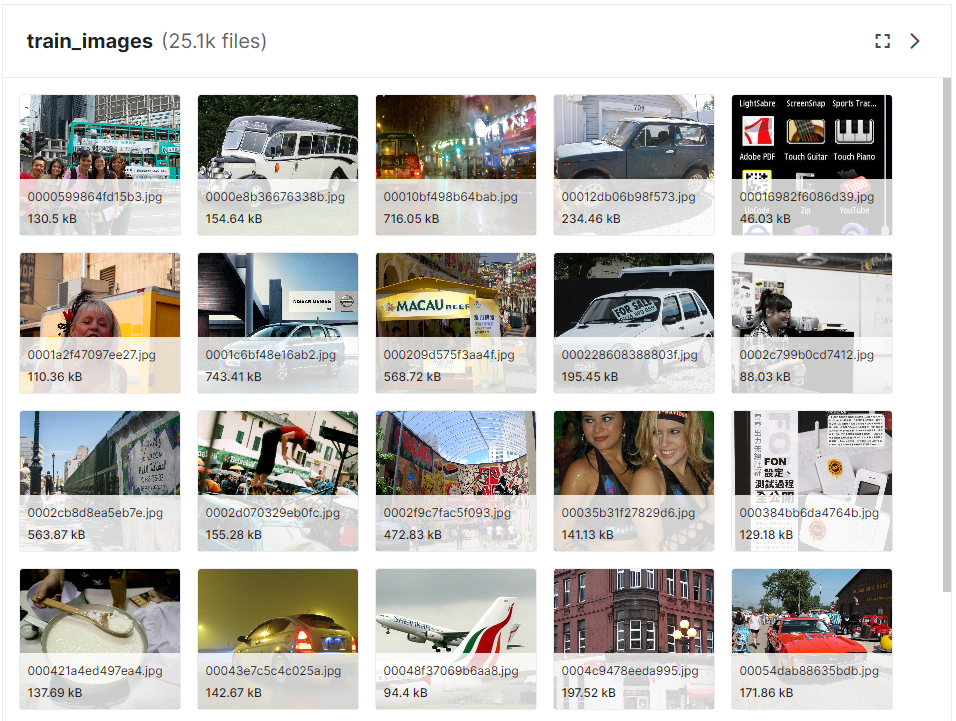
\includegraphics[scale=0.67]{images/Chapter3/text_ocr_dataset.png}}
\caption{Dataset 1: Text \acs{OCR} - Text Extraction from Images Dataset}
\label{textocrdataset}
\end {figure}

\newpage
\subsection{Dataset 2} \label{subsection:data2}
The second dataset is Sentiment analysis of \acs{OCR} text \cite{sentiocrkaggle}. It consists of 239 image files most of which have text inside them. After extracting the texts from these images, the sentiment of the text can be analyzed and they can be classified into either of three categories: positive, negative, or random. If the sentiment of the extracted text is positive, then it is categorized as 'positive' and if the sentiment detected is negative then the image is categorized as 'negative'. If the sentiment detected is neutral then it is categorized as 'random'. If the image does not have any text, then also it would be categorized as 'random' as there is no text whose sentiment is to be analyzed. Figure \ref{sentiocrdataset} shows a preview of the dataset:
\begin {figure}[ht]
\centering
\adjustbox{frame}{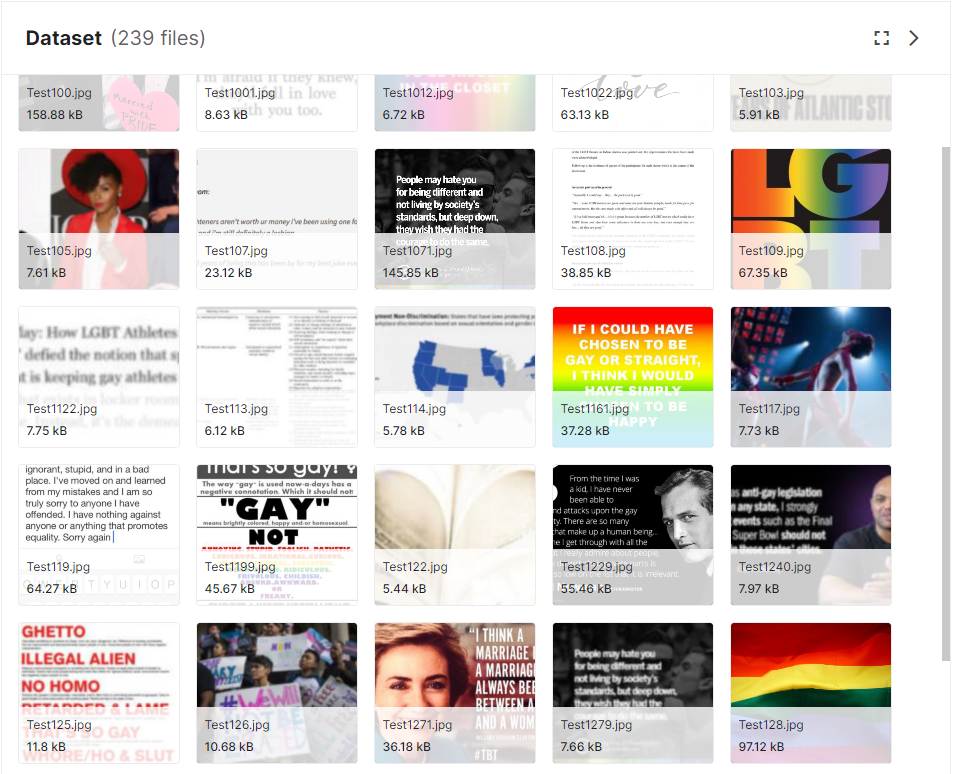
\includegraphics[scale=0.67]{images/Chapter3/senti_ocr_dataset.png}}
\caption{Dataset 2: Sentiment analysis of \acs{OCR} text Dataset}
\label{sentiocrdataset}
\end {figure}

\subsection{Dataset 3} \label{subsection:data3}
The third dataset is the \acs{DCA} Loan Dataset \cite{dcakaggle}. \ac{USAID} used \ac{DCA} \cite{dcalink} to issue loan guarantees.
This dataset contains private loans guaranteed under \acs{DCA} since 1999. It has information like guarantee numbers, location details, the size of the business, and so on. The list of columns and descriptions is mentioned in the table below.

\begin{table}[h]
\caption{Columns in \acs{DCA} dataset} 
\begin{center}
   
 \begin{tabular}{| p{5cm} | p{11cm} |}
   
\hline
 \textbf{Column Name} & \textbf{Description}\\ \hline \hline

     Guarantee Number &	Unique identifier for the loan guarantee. (String)\\ \hline
     Guarantee Country Name & Name of the country in which the loan was issued. (String)\\ \hline
     Amount (USD) & Name of the country in which the loan was issued. (String)\\ \hline
     Currency Name & Name of the currency in which the loan was issued. (String)\\ \hline
     End Date & Date when the loan term ends. (Date)\\ \hline
     Business Sector & Business sector in which the loan was issued. (String)\\ \hline
     City/Town & City or town in which the borrower is located. (String)\\ \hline
     State/Province/Region Name & Name of the state, province, or region in which the loan was issued. (String)\\ \hline
     State/Province/Region Code & Code of the state, province, or region in which the loan was issued. (String)\\ \hline
     State/Province/Region Country Name & Name of the country in which the state, province, or region is located. (String)\\ \hline
     Latitude & Latitude of the investment activity area. (Float)\\ \hline
     Longitude & Longitude of the investment activity area. (Float)\\ \hline
     Is Woman Owned? & Indicates whether the business is owned by a woman. (Boolean)\\ \hline
     Is First Time Borrower? & Indicates whether the borrower is a first-time borrower. (Boolean)\\ \hline
     Business Size & Size of the business associated with the loan. (String)\\ \hline

\end{tabular}                          
\label{dcadatasetcolumn}   
\end{center}
\end{table}

Figure \ref{dcaloandataset} shows a small snapshot of the dataset. A more clear image of the dataset can be found in Appendix \ref{dcaloandataset1} and \ref{dcaloandataset2}.
\begin {figure}[ht]
\centering
\adjustbox{frame}{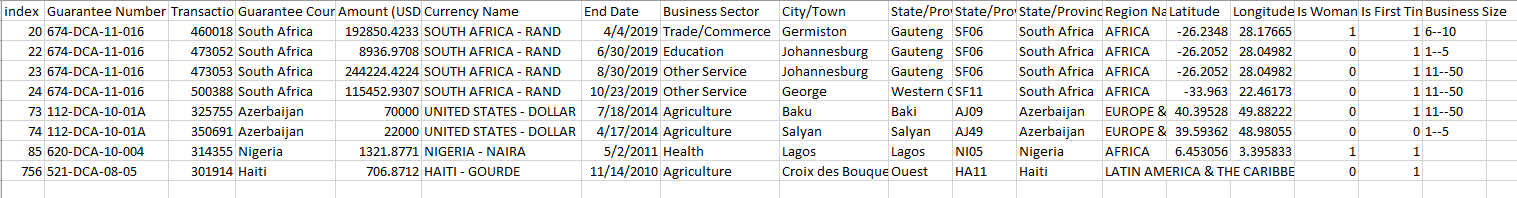
\includegraphics[scale=0.422]{images/Chapter3/dca_dataset.png}}
\caption{Dataset 3: \acs{DCA} Loan Dataset}
\label{dcaloandataset}
\end {figure}

\newpage
\subsection{Dataset 4} \label{subsection:data4}
The fourth dataset is Twitter Sentiment Dataset \cite{sentikaggle}. This was added because some of the cloud service providers did not accept image files as input for sentiment analysis. It consists of 162980 tweets; which are either of positive, neutral, or negative sentiment. The dataset was labeled. So first separated the labels and made only the tweets available in the input file. It was further necessary to convert the inputs into .txt files as Azure Language Studio accepted .txt files. Separated each tweet into a new text file and made a set of text files. Made a smaller sample of the dataset as there was an input character limitation of 5000 characters for processing. Figure \ref{sentidataset} shows a preview of the dataset:
\begin {figure}[ht]
\centering
\adjustbox{frame}{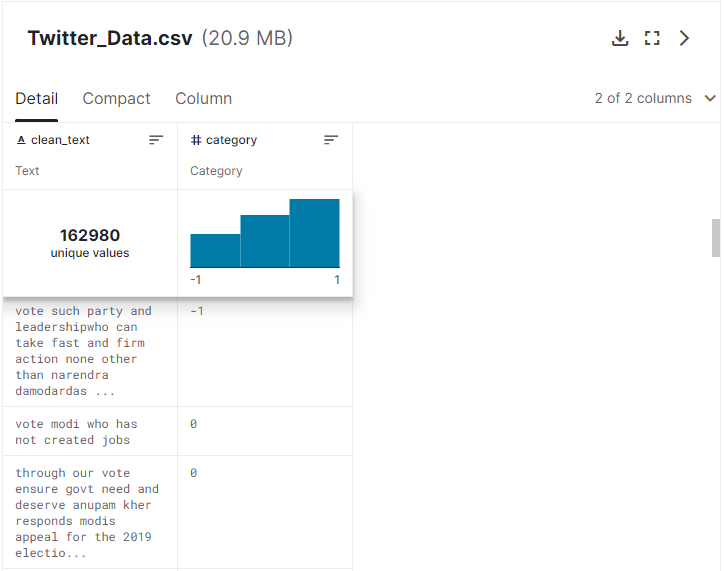
\includegraphics[scale=0.8]{images/Chapter3/senti_dataset4.png}}
\caption{Dataset 4: Twitter Sentiment Dataset}
\label{sentidataset}
\end {figure}

\section{Comparison/Evaluation Matrix}
\label{section:matrix}
\paragraph\ After doing the literature research the following evaluation metrics were selected to be tested against the datasets described above. Having added these metrics to the skeleton of the evaluation matrix, the table now looks like \ref{emptytable}. 

\begin{table}[h]
\caption{Evaluation matrix with metrics} 
\begin{center}
   
 \begin{tabular}{| p{3.45cm} || p{2.7cm} | p{3.5cm} | p{1.8cm} | p{3cm} |}
   
\hline
 \textbf{Service Provider} & \textbf{IBM Watson NLU} & \textbf{Microsoft Azure Cognitive \hspace{1cm}Services} & \textbf{Amazon Textract} & \textbf{Google Cloud Natural \hspace{1cm} Language}\\ \hline \hline 

     \acs{PII} detection & xyz & xyz & xyz & xyz\\ \hline
     Entity Recognition & xyz & xyz & xyz & xyz\\ \hline
     Sentiment Analysis & xyz & xyz & xyz & xyz\\ \hline
     Summarization & xyz & xyz & xyz & xyz\\ \hline
     Classification & xyz & xyz & xyz & xyz\\ \hline
     \acs{OCR} & xyz & xyz & xyz & xyz\\ \hline
     Free trial for users & xyz & xyz & xyz & xyz\\ \hline
     Documentation to use the service & xyz & xyz & xyz & xyz\\ \hline

\end{tabular}                          
\label{emptytable}   
\end{center}
\end{table}

A brief description of the metrics is provided below:
\begin{itemize}
    \item \acs{PII} detection: This feature lists all the details and information that have the capacity to identify an individual. Some examples of this are name, account number, social security number, phone number, email id, etc.
    \item Entity Recognition: This is a feature where information is located where an entity is mentioned. This can be used for classification purposes as well. Entities could be person names, cities, organizations, occupations, skills, etc.
    \item Summarization: The feature of condensing the given information concisely while preserving the essential meaning. 
    \item Classification: The feature of classifying or categorizing information into categories.
    \item \acs{OCR}: This features extracts all textual information from images. It could be from images of a handwritten text, from a scanned document, or even some writing (text) on a billboard in a scenic photograph.
    \item Free trial for users: This metric is to differentiate explicitly for services that provide free trial/limited access to their services without forcing the user to add a payment method.
    \item Documentation to use the service: As the field is relatively new, it is important to have guides/documents to guide the user through the portal initially. The availability of such documentation is stated in this metric.
\end{itemize}